%% This documentation was generated with Faust version 0.9.46
%% Wed Oct 15 22:37:51 2014
%% http://faust.grame.fr

\documentclass{article}

\usepackage[utf8]{inputenc}
\usepackage{graphicx}
\usepackage[usenames]{color}
\usepackage{listings}
\usepackage{supertabular}
\usepackage{amsmath}
\usepackage{latexsym, amssymb}
\usepackage{breqn}

% No indent
\setlength{\parindent}{0pt}

% Make LaTeX output a dot when typing an asterisk
\DeclareMathSymbol{*}{\mathbin}{symbols}{"01}

% lstlistings setup
\definecolor{yobg}{rgb}{0.9,0.9,1}
\definecolor{yotxt}{rgb}{0.01,0.01,0.52} % a dark blue.
\definecolor{mylstbg}{rgb}{0.98,0.98,0.98} % a really pale grey.
\definecolor{mylstcmt}{rgb}{0.01,0.52,0.01} % a dark green.
\definecolor{mylstdoc}{rgb}{0.80,0.30,0.80} % a medium pink.

\lstset{%
  language=C++, 
  numbers=left,%none,
  tabsize=4, 
  frame=single, 
  breaklines=true, 
  numberstyle=\tiny\ttfamily, 
  backgroundcolor=\color{mylstbg}, 
  basicstyle=\scriptsize\ttfamily, 
  commentstyle=\slshape\color{mylstcmt}, %\itshape,
  frameround=tttt, 
  columns=flexible, %fixed, 
  showstringspaces=false,
  emptylines=2,
  inputencoding=utf8,
  extendedchars=true,
  literate=	{á}{{\'a}}1 
			{à}{{\`a}}1 
			{ä}{{\"a}}1 
			{â}{{\^a}}1
			{é}{{\'e}}1 
			{è}{{\`e}}1 
			{ë}{{\"e}}1 
			{ê}{{\^e}}1
			{ï}{{\"i}}1 
			{î}{{\^i}}1
			{ö}{{\"o}}1 
			{ô}{{\^o}}1
			{è}{{\`e}}1 
			{ù}{{\`u}}1 
			{û}{{\^u}}1
			{ç}{{\c{c}}}1 
			{Ç}{{\c{C}}}1,
  emph={component, declare, environment, import, library, process},
  emph={[2]ffunction, fconstant, fvariable},
  emph={[3]button, checkbox, vslider, hslider, nentry, vgroup, hgroup, tgroup, vbargraph, hbargraph, attach},
  emphstyle=\color{yotxt}, %\underline, %\bfseries,
  morecomment=[s][\color{mylstdoc}]{<mdoc>}{</mdoc>},
  rulecolor=\color{black}
}

\newcommand{\faustfilename}{Sinewaveoscillator.dsp}
\newcommand{\faustdocdir}{Sinewaveoscillator-mdoc}
\newcommand{\faustprogname}{Sinewaveoscillator}
\newcommand{\faustversion}{0.9.46}
\newcommand{\faustdocdate}{October 15, 2014}

\begin{document}
\title{Sinewaveoscillator}
\date{\today}
\maketitle
\begin{tabular}{ll}
	\hline
	\textbf{math.lib/name} & Math Library \\
	\textbf{math.lib/author} & GRAME \\
	\textbf{math.lib/copyright} & GRAME \\
	\textbf{math.lib/version} & 1.0 \\
	\textbf{math.lib/license} & LGPL \\
	\hline
\end{tabular}
\bigskip

\bigskip
This document provides a mathematical description of the Faust program text stored in the \texttt{\faustfilename} file. See the notice in Section\,\ref{notice} (page\,\pageref{notice}) for details.


\section{Mathematical definition of \texttt{process}}
\label{equation}

The \emph{\faustprogname} program evaluates the signal transformer denoted by \texttt{process}, which is mathematically defined as follows:

% Set of Faust formulas (corresponding to an <equation> tag).
\begin{enumerate}

\item Output signal $y$ such that
	\begin{dgroup*}
		\begin{dmath*}
				y(t) = r_{1}(t)
		\end{dmath*}
	\end{dgroup*}

\item Input signal (none)

\item Intermediate signals  $r_i$ for $i \in [1,2]$ such that
	\begin{dgroup*}
		\begin{dmath*}
				r_{2}(t) = r_{1}(t\!-\!1) *  \left(r_{1}(t\!-\!1) \hiderel{\neq} 1\right) 
		\end{dmath*}
		\begin{dmath*}
				r_{1}(t) = k_{1} + r_{2}(t\!-\!1)
		\end{dmath*}
	\end{dgroup*}

\item Constant $k_1$ such that
	\begin{dgroup*}
		\begin{dmath*}
				k_{1} = \min\left( 0.05 * \min\left( 192000, \max\left( 1, f_S \right) \right), 1 \right)
		\end{dmath*}
	\end{dgroup*}

\end{enumerate}


\section{Block diagram of \texttt{process}}
\label{diagram}

The block diagram of \texttt{process} is shown on Figure\,\ref{figure1} (page\,\pageref{figure1}).
\begin{figure}[ht!]
	\centering
	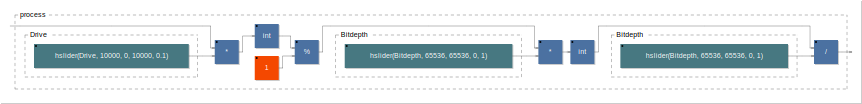
\includegraphics[width=\textwidth]{../svg/svg-01/process}
	\caption{Block diagram of \texttt{process}}
	\label{figure1}
\end{figure}


\section{Notice}
\label{notice}


\begin{itemize}
	\item This document was generated using Faust version \faustversion\ on \faustdocdate.
	\item The value of a Faust program is the result of applying the signal transformer denoted by the expression to which the \texttt{process} identifier is bound to input signals, running at the $f_S$ sampling frequency.
	\item Faust (\emph{Functional Audio Stream}) is a functional programming language designed for synchronous real-time signal processing and synthesis applications. A Faust program is a set of bindings of identifiers to expressions that denote signal transformers. A signal $s$ in $S$ is a function mapping\footnote{Faust assumes that $\forall \, s \in S, \forall \, t \in \mathbb{Z}, s(t) = 0 \mathrm{\ when\ } t < 0$.} times $t \in \mathbb{Z}$ to values $s(t) \in \mathbb{R}$, while a signal transformer is a function from $S^n$ to $S^m$, where $n,m\in \mathbb{N}$. See the Faust manual for additional information (\textsf{http://faust.grame.fr}).
	\item Every mathematical formula derived from a Faust expression is assumed, in this document, to having been normalized (in an implementation-depen\-dent manner) by the Faust compiler.
	\item A block diagram is a graphical representation of the Faust binding of an identifier I to an expression E; each graph is put in a box labeled by I. Subexpressions of E are recursively displayed as long as the whole picture fits in one page.
	\item The \texttt{\faustdocdir/} directory may also include the following subdirectories:
\begin{itemize}
	\item	\texttt{cpp/} for Faust compiled code; 
	\item	\texttt{pdf/} which contains this document; 
	\item	\texttt{src/} for all Faust sources used (even libraries); 
	\item	\texttt{svg/} for block diagrams, encoded using the Scalable Vector Graphics format (\textsf{http://www.w3.org/Graphics/SVG/});
	\item	\texttt{tex/} for the \LaTeX\ source of this document.
\end{itemize}
\end{itemize}


\section{Faust code listings}
\label{listing}

This section provides the listings of the Faust code used to generate this document, including dependencies.

\bigskip\bigskip
\begin{lstlisting}[caption=\texttt{Sinewaveoscillator.dsp}]
import("math.lib");
loop(begin, eind, tijdinms)=
(_+((eind - begin)/tijdinms:max(1):min(SR/20)))~(((_<:(begin*(_==eind),_*(_!=eind):_+_)))@(1)):

_;

BitDepth=_/2^(8*checkbox("8 or 16 bit")+ 1):_;
sine=_*(2*PI):sin:_;
process = loop(0, 1, 100);//BitDepth:sine;

//((eind - begin)/tijdinms:max(1):min(SR/20))
\end{lstlisting}


\bigskip\bigskip
\begin{lstlisting}[caption=\texttt{math.lib}]
/************************************************************************
 ************************************************************************
  	FAUST library file
	Copyright (C) 2003-2011 GRAME, Centre National de Creation Musicale
    ---------------------------------------------------------------------
    This program is free software; you can redistribute it and/or modify
    it under the terms of the GNU Lesser General Public License as 
	published by the Free Software Foundation; either version 2.1 of the 
	License, or (at your option) any later version.

    This program is distributed in the hope that it will be useful,
    but WITHOUT ANY WARRANTY; without even the implied warranty of
    MERCHANTABILITY or FITNESS FOR A PARTICULAR PURPOSE.  See the
    GNU Lesser General Public License for more details.

    You should have received a copy of the GNU Lesser General Public
 	License along with the GNU C Library; if not, write to the Free
  	Software Foundation, Inc., 59 Temple Place, Suite 330, Boston, MA
  	02111-1307 USA. 
 ************************************************************************
 ************************************************************************/

declare name "Math Library";
declare author "GRAME";
declare copyright "GRAME";
declare version "1.0";
declare license "LGPL"; 

//--------------------------------------------------------------------------------
// 						Mathematic library for Faust

// Implementation of the math.h file as Faust foreign functions
//
// History
// ----------
// 28/06/2005	[YO]	postfixed functions with 'f' to force float version
//						instead of double
//			  	[YO]	removed 'modf' because it requires a pointer as argument
//---------------------------------------------------------------------------------

// -- Utilities and constants

SR 			= min(192000, max(1, fconstant(int fSamplingFreq, <math.h>)));
BS          = fvariable(int count, <math.h>);

PI          = 3.1415926535897932385;

// -- neg and inv functions

neg(x)      = -x;
inv(x)      = 1/x;

// -- Trigonometric Functions

//acos		= ffunction(float acosf (float), <math.h>, "");
//asin		= ffunction(float asinf (float), <math.h>, "");
//atan		= ffunction(float atanf (float), <math.h>, "");
//atan2		= ffunction(float atan2f (float, float), <math.h>, "");

//sin			= ffunction(float sinf (float), <math.h>, "");
//cos			= ffunction(float cosf (float), <math.h>, "");
//tan			= ffunction(float tanf (float), <math.h>,"");

// -- Exponential Functions

//exp 		= ffunction(float expf (float), <math.h>,"");
//log 		= ffunction(float logf (float), <math.h>,"");
//log10 	= ffunction(float log10f (float), <math.h>,"");
//pow 		= ffunction(float powf (float, float), <math.h>,"");
//sqrt 		= ffunction(float sqrtf (float), <math.h>,"");
cbrt 		= ffunction(float cbrtf (float), <math.h>,"");
hypot 		= ffunction(float hypotf (float, float), <math.h>,"");
ldexp 		= ffunction(float ldexpf (float, int), <math.h>,"");
scalb 		= ffunction(float scalbf (float, float), <math.h>,"");
log1p 		= ffunction(float log1pf (float), <math.h>,"");
logb 		= ffunction(float logbf (float), <math.h>,"");
ilogb 		= ffunction(int ilogbf (float), <math.h>,"");
expm1 		= ffunction(float expm1f (float), <math.h>,"");

// -- Hyperbolic Functions

acosh		= ffunction(float acoshf (float), <math.h>, "");
asinh		= ffunction(float asinhf (float), <math.h>, "");
atanh		= ffunction(float atanhf (float), <math.h>, "");

sinh		= ffunction(float sinhf (float), <math.h>, "");
cosh		= ffunction(float coshf (float), <math.h>, "");
tanh		= ffunction(float tanhf (float), <math.h>,"");

// -- Remainder Functions

//fmod 		= ffunction(float fmodf (float, float),<math.h>,"");
//remainder 	= ffunction(float remainderf (float, float),<math.h>,"");

// -- Nearest Integer Functions

//floor 		= ffunction(float floorf (float), <math.h>,"");
//ceil 		= ffunction(float ceilf (float), <math.h>,"");
//rint 		= ffunction(float rintf (float), <math.h>,"");

// -- Special Functions

erf			= ffunction(float erff(float), <math.h>,"");
erfc		= ffunction(float erfcf(float), <math.h>,"");
gamma		= ffunction(float gammaf(float), <math.h>,"");
J0			= ffunction(float j0f(float), <math.h>,"");
J1			= ffunction(float j1f(float), <math.h>,"");
Jn			= ffunction(float jnf(int, float), <math.h>,"");
lgamma		= ffunction(float lgammaf(float), <math.h>,"");
Y0			= ffunction(float y0f(float), <math.h>,"");
Y1			= ffunction(float y1f(float), <math.h>,"");
Yn			= ffunction(float ynf(int, float), <math.h>,"");


// -- Miscellaneous Functions

//fabs 		= ffunction(float fabsf (float), <math.h>,"");
//fmax 		= ffunction(float max (float, float),<math.h>,"");
//fmin 		= ffunction(float min (float, float),<math.h>,"");

fabs = abs;
fmax = max;
fmin = min;

isnan 		= ffunction(int isnan (float),<math.h>,"");
nextafter	= ffunction(float nextafter(float, float),<math.h>,"");

// Pattern matching functions to count and access the elements of a list
// USAGE : 	count ((10,20,30,40)) 	-> 4  
//			take  (3,(10,20,30,40)) -> 30
// 

count ((xs, xxs)) = 1 + count(xxs);
count (xx) = 1;

take (1, (xs, xxs)) 	= xs;
take (1, xs) 			= xs;
take (nn, (xs, xxs)) 	= take (nn-1, xxs);

// linear interpolation between two signals 
interpolate(i) = *(1.0-i),*(i) : +; 

// if-then-else implemented with a select2. 
if(cond,thn,els) = select2(cond,els,thn);


//-----------------------------------------------------------------
// countdown(count,trig) 
// start counting down from count, count-1,...,0 when trig > 0
//-----------------------------------------------------------------
countdown(count, trig)	= \(c).(if(trig>0, count, max(0, c-1))) ~_;

//-----------------------------------------------------------------
// countup(count,trig) 
// start counting down from 0, 1, ... count-1, count when trig > 0
//-----------------------------------------------------------------
countup(count, trig)	= \(c).(if(trig>0, 0, min(count, c+1))) ~_;

/******************************************************************
 *  Hadamard matrix function
 *  Implementation contributed by Remy Muller
 *****************************************************************/

// bus(n) : n parallel cables
bus(2) = _,_; // avoids a lot of "bus(1)" labels in block diagrams
bus(n) = par(i, n, _);

// selector(i,n) : select ith cable among n
selector(i,n) = par(j, n, S(i, j))    with { S(i,i) = _; S(i,j) = !; };

// interleave(m,n) : interleave m*n cables : x(0), x(m), x(2m), ..., x(1),x(1+m), x(1+2m)...
//interleave(m,n) = bus(m*n) <: par(i, m, par(j, n, selector(i+j*m,m*n))); 

// interleave(row,col) : interleave row*col cables from column order to row order.
// input : x(0), x(1), x(2) ..., x(row*col-1)
// output: x(0+0*row), x(0+1*row), x(0+2*row), ..., x(1+0*row), x(1+1*row), x(1+2*row), ...
interleave(row,col) = bus(row*col) <: par(r, row, par(c, col, selector(r+c*row,row*col))); 

// butterfly(n) : addition then substraction of interleaved signals : 
butterfly(n) = bus(n) <: interleave(n/2,2), interleave(n/2,2) : par(i, n/2, +), par(i, n/2, -);

// hadamard(n) : hadamard matrix function of size n = 2^k
hadamard(2) = butterfly(2);
hadamard(n) = butterfly(n) : (hadamard(n/2) , hadamard(n/2));
\end{lstlisting}


\end{document}

